\pdfminorversion=4
\documentclass[aspectratio=169]{beamer}

\mode<presentation>
{
  \usetheme{default}
  \usecolortheme{default}
  \usefonttheme{default}
  \setbeamertemplate{navigation symbols}{}
  \setbeamertemplate{caption}[numbered]
  \setbeamertemplate{footline}[frame number]  % or "page number"
  \setbeamercolor{frametitle}{fg=white}
  \setbeamercolor{footline}{fg=black}
} 

\usepackage[english]{babel}
\usepackage{inputenc}
\usepackage{tikz}
\usepackage{courier}
\usepackage{array}
\usepackage{bold-extra}
\usepackage{minted}
\usepackage[thicklines]{cancel}
\usepackage{fancyvrb}
\usepackage{halloweenmath}

\xdefinecolor{ucred}{rgb}{0.50,0,0}
\xdefinecolor{dianablue}{rgb}{0.18,0.24,0.31}
\xdefinecolor{darkblue}{rgb}{0.1,0.1,0.7}
\xdefinecolor{darkgreen}{rgb}{0,0.5,0}
\xdefinecolor{darkgrey}{rgb}{0.35,0.35,0.35}
\xdefinecolor{darkorange}{rgb}{0.8,0.5,0}
\xdefinecolor{darkred}{rgb}{0.7,0,0}
\definecolor{darkgreen}{rgb}{0,0.6,0}
\definecolor{mauve}{rgb}{0.58,0,0.82}

\title[2025-10-31-oaec-foundgully-with-adam]{\textcolor{black}{Detecting gullies in LIDAR bare earth elevation data}}
\author{Jim Pivarski}
\institute{University of Chicago -- Data Science Institute}
\date{October 31, 2025 $\bigpumpkin$}

\usetikzlibrary{shapes.callouts}

\begin{document}

\logo{\pgfputat{\pgfxy(0.11, 7.4)}{\pgfbox[right,base]{\tikz{\filldraw[fill=ucred, draw=none] (0 cm, 0 cm) rectangle (50 cm, 1 cm);}\mbox{\hspace{-8 cm}
\includegraphics[height=1 cm]{uchicago-logo-long.png}\hspace{0.1 cm}{
\includegraphics[height=1 cm]{dsi-logo-long.png}}\hspace{0.1 cm}}}}}

\begin{frame}
  \titlepage
\end{frame}

\logo{\pgfputat{\pgfxy(0.11, 7.4)}{\pgfbox[right,base]{\tikz{\filldraw[fill=ucred, draw=none] (0 cm, 0 cm) rectangle (50 cm, 1 cm);}\mbox{\hspace{-8 cm}
\includegraphics[height=1 cm]{uchicago-logo.png}{
\includegraphics[height=1 cm]{dsi-logo.png}}\hspace{0.1 cm}}}}}

% Uncomment these lines for an automatically generated outline.
%\begin{frame}{Outline}
%  \tableofcontents
%\end{frame}

% START START START START START START START START START START START START START

\begin{frame}{What I found in the literature}
\large
\vspace{0.5 cm}

Several papers all described the same technique:
\begin{itemize}
\item draw images of small-scale variations in elevation by subtracting elevation at each point with the average of its neighbors.
\end{itemize}

\vspace{0.5 cm}
\begin{uncoverenv}<2->
\begin{center}
\begin{minipage}{0.75\linewidth}
Here's one:
\vspace{0.5 cm}

\centering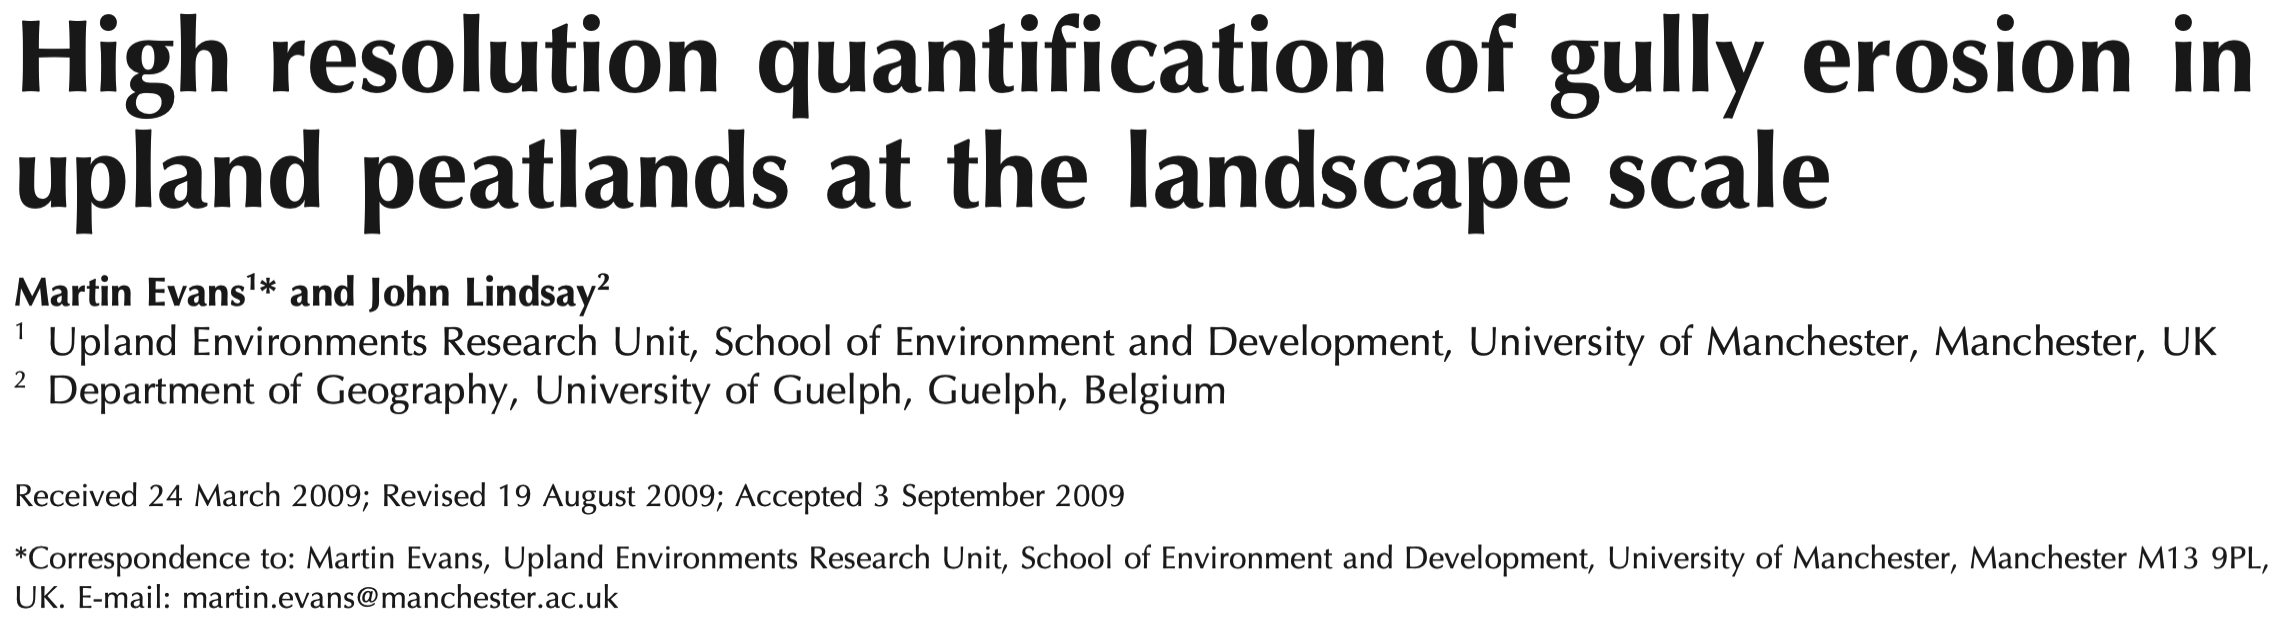
\includegraphics[width=\linewidth]{img/evans-lindsay-2010-gully-title.png}
\end{minipage}
\end{center}
\end{uncoverenv}
\end{frame}

\begin{frame}{What I found in the literature}
\vspace{0.5 cm}
\begin{columns}
\column{0.6\linewidth}
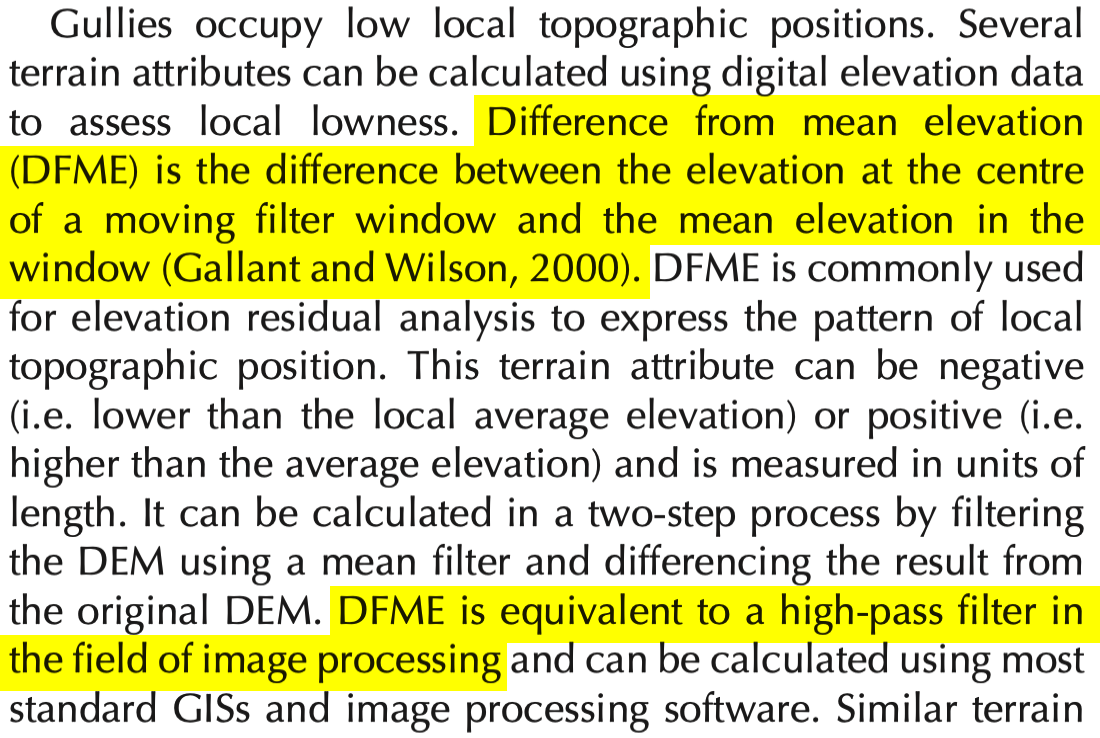
\includegraphics[width=\linewidth]{img/evans-lindsay-2010-gully-exerpt.png}

\column{0.4\linewidth}
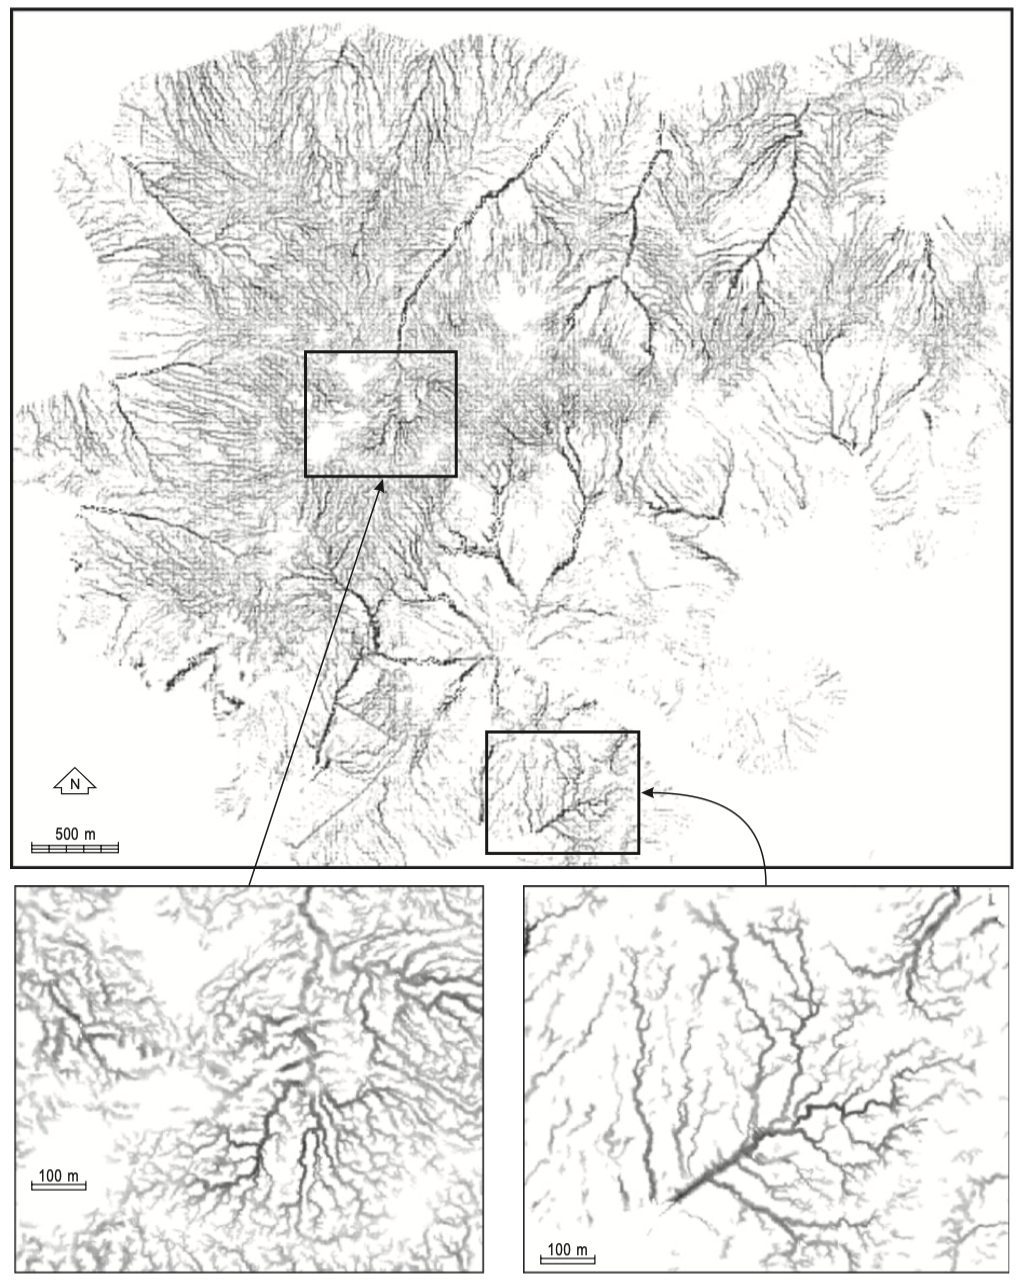
\includegraphics[width=\linewidth]{img/evans-lindsay-2010-gully-figure.png}
\end{columns}
\end{frame}

\begin{frame}{This procedure is a convolution with an appropriately defined kernel}
\vspace{0.15 cm}
\begin{center}
``Subtract each pixel from the average of a disk centered on that pixel.''

\vspace{0.25 cm}
is equivalent to

\vspace{0.25 cm}
``Convolve with a kernel that is positive in the center pixel, uniformly negative \\ in a disk around the pixel, zero elsewhere, and sums to zero.''

\vspace{0.35 cm}
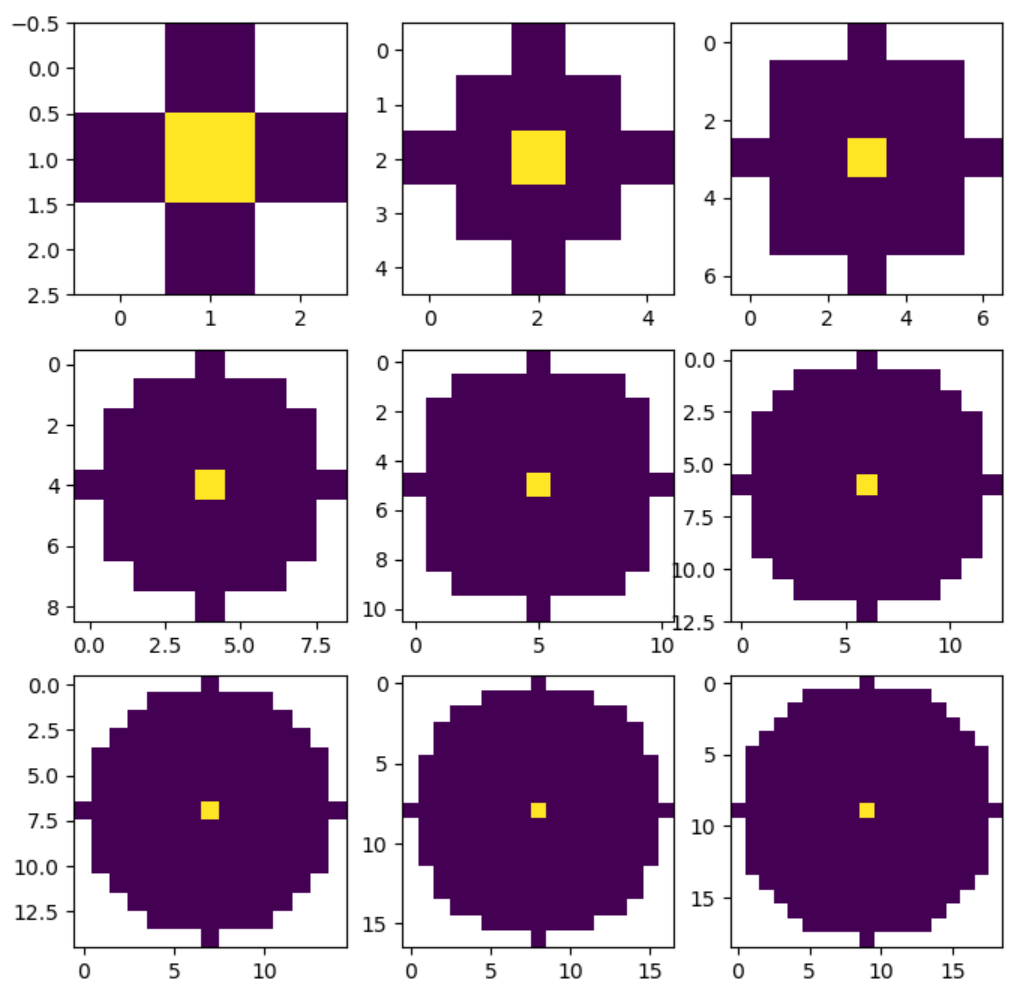
\includegraphics[width=0.35\linewidth]{img/simple-kernels.png}
\end{center}
\end{frame}

\begin{frame}{It works! Especially if the disk is very large}
\vspace{0.15 cm}
\centering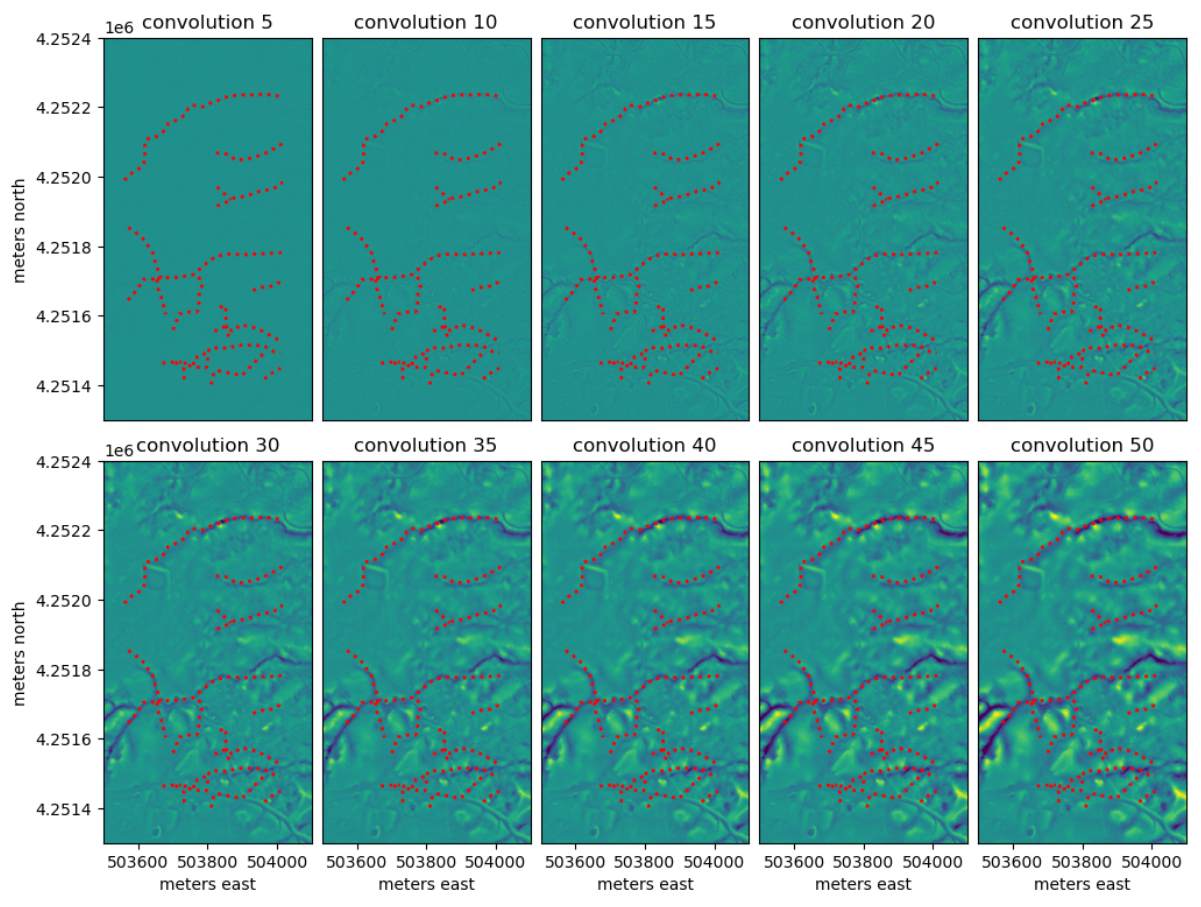
\includegraphics[width=0.75\linewidth]{img/first-convolution-results.png}
\end{frame}

\begin{frame}{But if a point-in-disk is good, wouldn't a line-in-disk be better?}
\vspace{0.5 cm}
\begin{columns}
\column{0.55\linewidth}
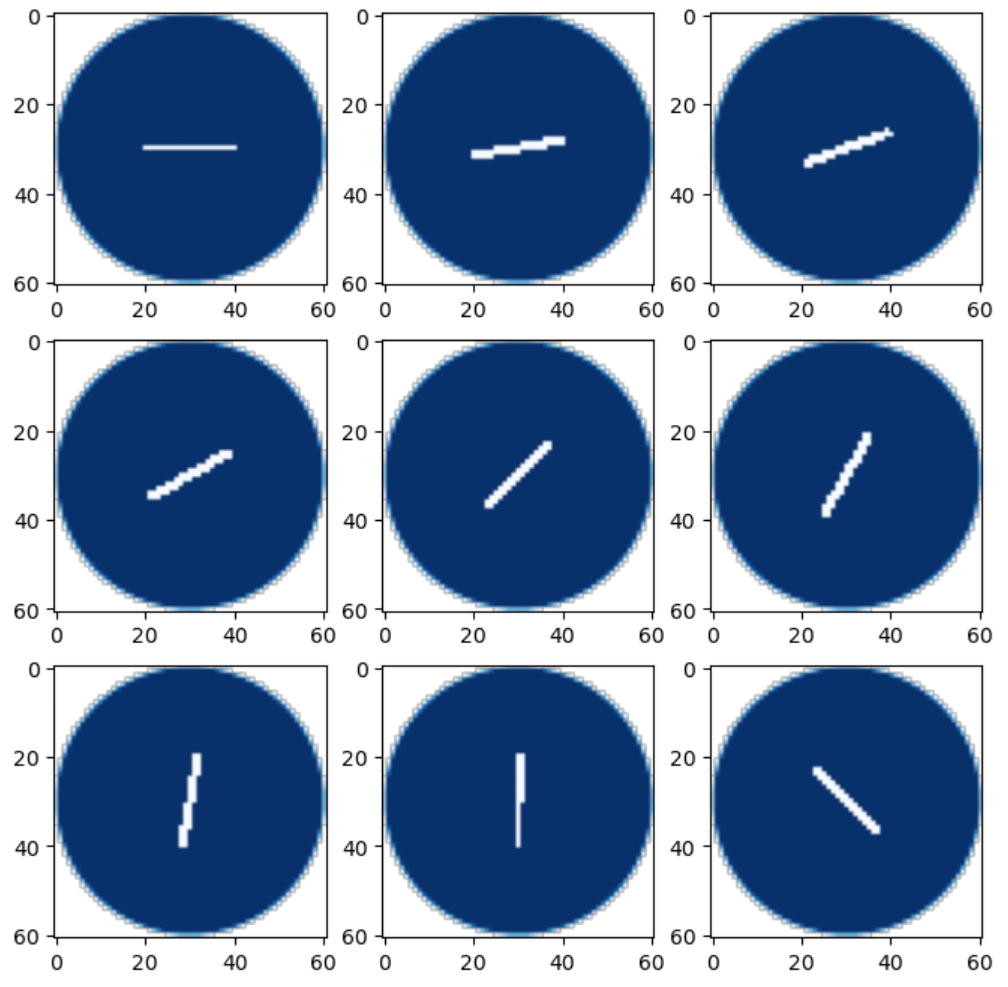
\includegraphics[width=\linewidth]{img/angled-convolution-kernels.png}

\column{0.45\linewidth}
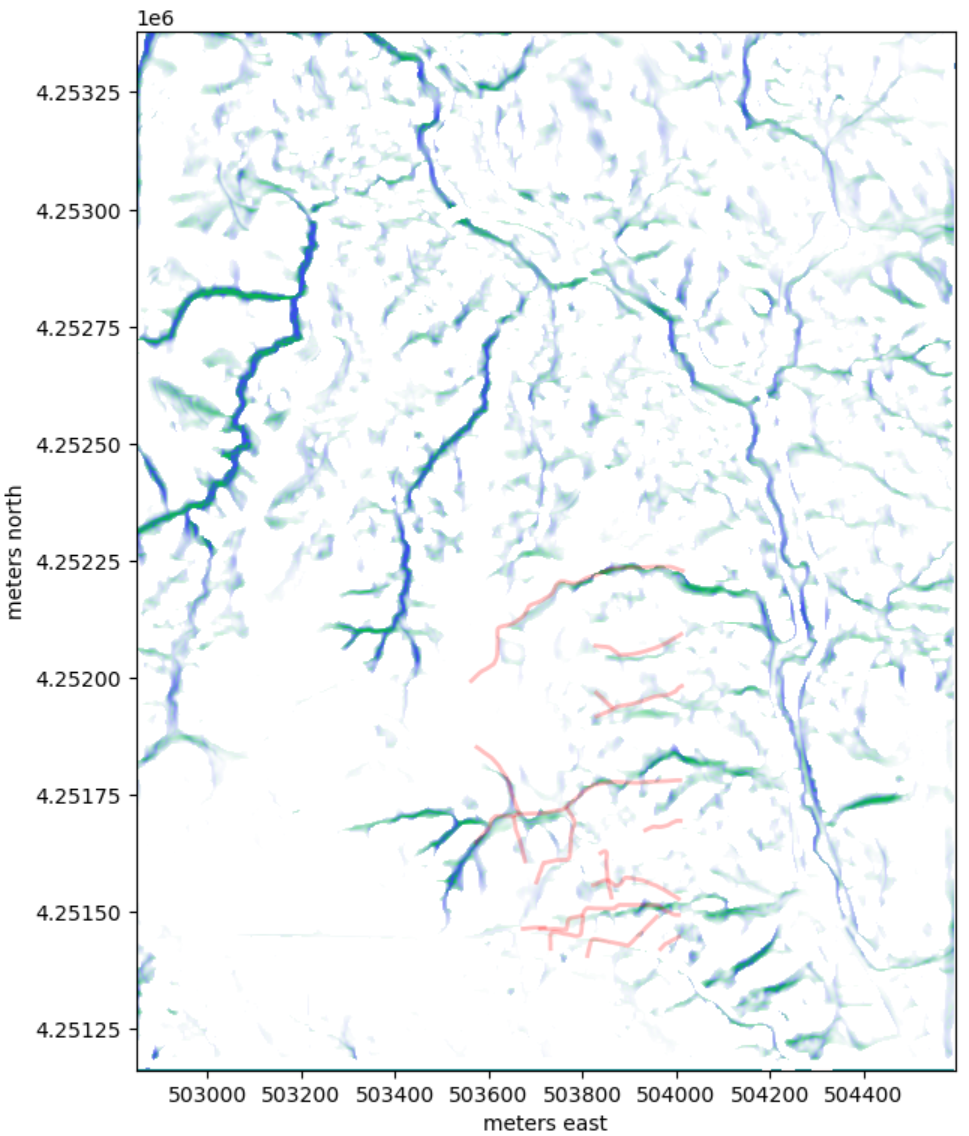
\includegraphics[width=\linewidth]{img/angled-convolution-results.png}

\end{columns}
\end{frame}

\begin{frame}{I studied the response of gully and non-gully pixels to various kernels}
\small
\vspace{0.5 cm}
\begin{columns}
\column{0.5\linewidth}
\begin{minipage}{0.5\linewidth}
\raggedright A refined {\bf line-in-disk kernel} in which the line is a Gaussian peak with width $\sigma$.

\vspace{0.15 cm}
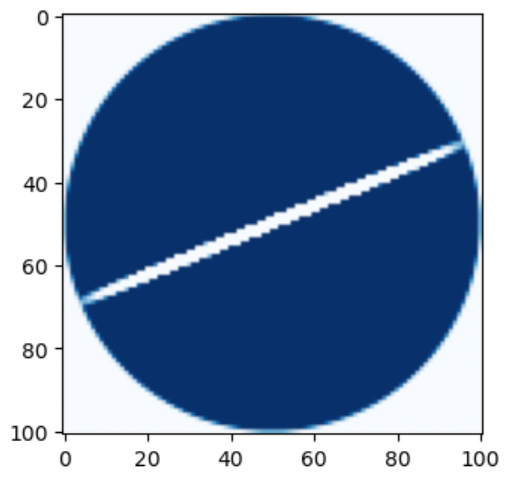
\includegraphics[width=\linewidth]{img/gaussian-line-in-disk-kernel.png}
\end{minipage}

\hfill \begin{minipage}{0.5\linewidth}
\vspace{-2.8 cm}
\raggedleft This {\bf cliff-edge kernel} responds best to a sharp drop in elevation, aligned with its angle.

\vspace{0.15 cm}
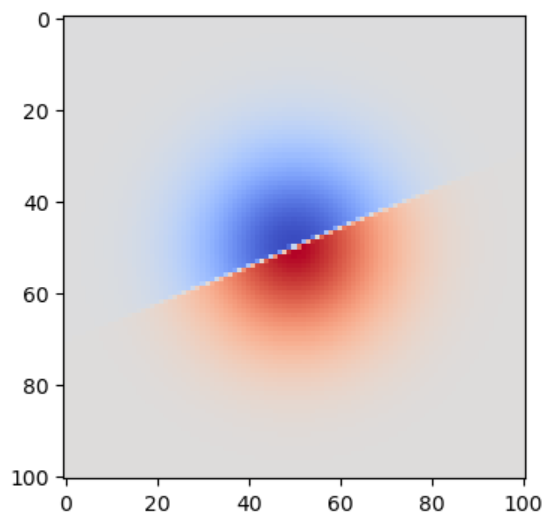
\includegraphics[width=\linewidth]{img/cliff-edge-kernel.png}
\end{minipage}

\column{0.5\linewidth}
Gully pixels respond best when the line-in-disk kernel's angle is aligned with the gully trough, and the parallel-versus-perpendicular response is biggest for the longest lines.

\vspace{0.25 cm}
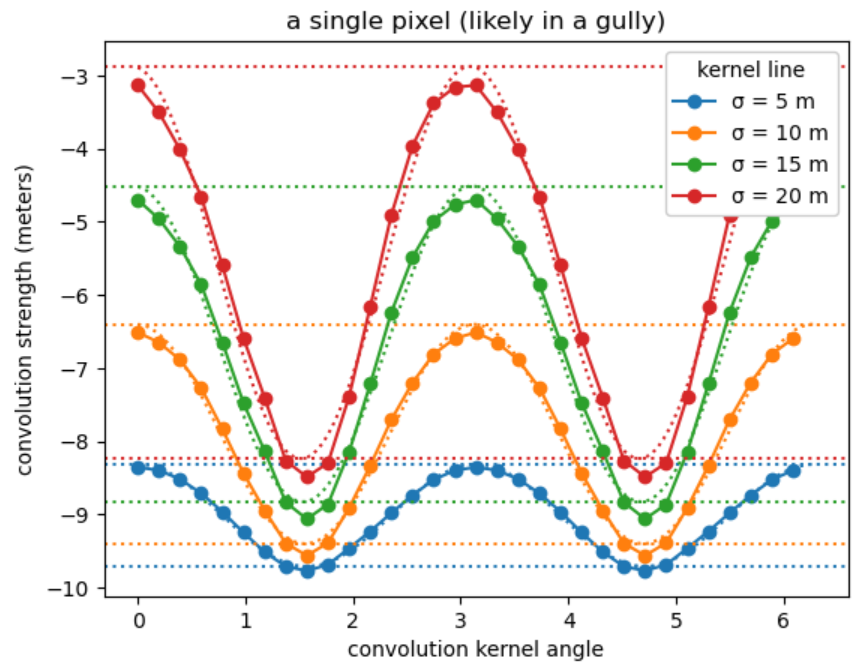
\includegraphics[width=\linewidth]{img/response-to-line-in-disk-convolution.png}
\end{columns}
\end{frame}

\begin{frame}{Optimizing a gully-finder model}
\vspace{0.25 cm}
\large
\begin{itemize}\setlength{\itemsep}{0.25 cm}
\item<1-> Maximum convolution response (maximized over angle) is a good indicator of being in a gully.
\item<2-> Minimum difference between high and low (varying angle) is a good indicator of {\it not} being in a gully.
\item<3-> Empirically, real gullies are a little more pointed than a sinusoidal fit.
\item<4-> The line-in-disk kernel matches one-sided cliff-edges too well, but the specialized cliff-edge kernel matches cliffs and not gullies, so it can be a veto.
\end{itemize}

\vspace{0.5 cm}
\uncover<5->{$\longrightarrow$ all of these can be features in an optimized model.}

\vspace{0.5 cm}
\uncover<6->{Since there's only a handful of features, it will be a linear fit.}
\end{frame}

\end{document}
